% -- Encoding UTF-8 without BOM
% -- XeLaTeX => PDF (BIBER)

\documentclass{cv-style}     % Add 'print' as an option into the square bracket to remove colours from this template for printing.

\setdefaultlanguage{french}
\sethyphenation{french}{} % Add words between the {} to avoid them to be cut

%----------------------------------------------------------------------------------------
%	Page layout
%----------------------------------------------------------------------------------------
\cvheadheight{3.5cm}
\cvasidewidth{4.7}
\cvasidevpos{3.5}
\cvmainwidth{11.5cm}
\geometry{left=6.4cm, top=2.5cm, right=1cm, bottom=1cm}

%----------------------------------------------------------------------------------------
%	Bibliography
%----------------------------------------------------------------------------------------
\usepackage[sectcntreset]{bibtopic}
\usepackage{natbib}
\bibliographystyle{bib/achemso_perso}
\AtBeginDocument{\nocite{achemso-control}}

%----------------------------------------------------------------------------------------
%	hyperlink setup
%----------------------------------------------------------------------------------------
\hypersetup{
    pdftitle=CV \textbar{} Germain Vallverdu,%
    pdfauthor=Germain Vallverdu
}

%----------------------------------------------------------------------------------------
%	Setup las updated text
%----------------------------------------------------------------------------------------
%\lastupdated{Mise à jour le \today}

%----------------------------------------------------------------------------------------
%	Add a few custom packages
%----------------------------------------------------------------------------------------
\usepackage{fontawesome}

\begin{document}

\header{Germain }{Salvato Vallverdu}{Maître de conférences -- Docteur en Chimie-Physique}          % Your name
%\lastupdated

%----------------------------------------------------------------------------------------
%	SIDEBAR SECTION  -- In the aside, each new line forces a line break
%----------------------------------------------------------------------------------------

\begin{aside}
    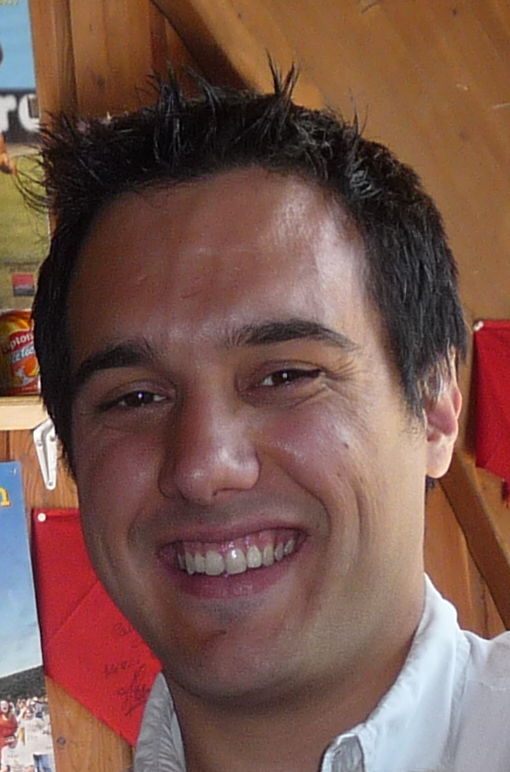
\includegraphics[width=.8\columnwidth]{img/germain}
    10 août 1983, France
    Marié, 2 enfants
    %
    \section{Contact}
    germain.vallverdu@univ-pau.fr
    05 59 40 78 51
    06 88 59 08 87
    ~
    IPREM
    Technopôle Hélioparc
    2 ave du Président P. Angot
    64053 Pau cedex 9
    %
    \section{Chimie Théorique}
    Modélisation
    Développement
    Stratégies calculatoires
    VASP, CRYSTAL (solide)
    Gaussian (molécule)
    DL-POLY, AMBER (dynamique)
    %
    \section{Programmation}
    Fortran, C
    Python
    \LaTeX{}, HTML/CSS
    %
    \section{Langues}
    Français
    Anglais (Professional)
    %
    \section{Sur internet}
    \href{http://orcid.org/0000-0003-1116-8776}{$\vcenter{\hbox{
\includegraphics{img/iD-icon}}}$ orcid.org/0000-0003-1116-8776}
    %\href{https://github.com/gVallverdu}{$\vcenter{\hbox{
\includegraphics[height=16pt]{img/GitHub-Mark}}}$ gVallverdu}
    \href{https://github.com/gVallverdu}{\faGithub{} gVallverdu}
    \href{http://gvallver.perso.univ-pau.fr}{\faGlobe{} gvallver.perso.univ-pau.fr}
    %
\end{aside}

\section{Rés}{umé}

Physico-chimiste de formation, je suis Maître de conférences en chimie théorique
 à l'Université de Pau et des Pays de l'Adour à l'IPREM (Institut des sciences
 analytiques et de Physico-chimie pour l'environnement et les matériaux). Mes activités de
recherche concernent le développement et l'utilisation de méthodes de simulations
numériques à
différentes échelles de temps et ou d'espace, appliquées
à l'étude de systèmes complexes. J'effectue mes enseignements à l'UFR sciences et
techniques de Pau principalement en chimie-physique.

\section{Experience}{ Professionnelle}

\begin{entrylist}
%------------------------------------------------
\entry
  {depuis 2010~}
  {Université de Pau et des Pays de l'Adour}
  {Pau, France}
  {\jobtitle{Maître de conférences}\\
   Chimie théorique et simulation numérique.
   Surface, interface et réactivité.}
%------------------------------------------------
\entry
  {2009--2010}
  {CEA - DAM}
  {Bruyères le châtel, France}
  {
  \jobtitle{Chercheur-ingénieur}\\
  Développement et implémentation d'un modèle mésoscopique pour l'étude de la propagation
  d'ondes de chock réactives dans un système hétérogène.
  }
%------------------------------------------------
\entry
  {2006--2009}
  {Université Paris-Sud 11}
  {Orsay, France}
  {
  \jobtitle{Allocataire de recherche, moniteur}\\
  Étude théorique de processus photophysiques dans les protéines fluorescentes.
  }
%------------------------------------------------
\end{entrylist}

%----------------------------------------------------------------------------------------
%	EDUCATION SECTION
%----------------------------------------------------------------------------------------

\section{Form}{ation}

\begin{entrylist}
%------------------------------------------------
\entry
{2006-2009}
{Doctorat de chimie {\normalfont spécialité chimie-théorique}}
{Université Paris-Sud 11}
{Mention très honorable}
%------------------------------------------------
\entry
{2004-2006}
{Master de chimie {\normalfont spécialité physico-chimie moléculaire}}
{Université Paris-Sud 11}
{Mention TB}
%------------------------------------------------
\entry
{2003-2004}
{Licence de chimie-physique}
{Université Paris-Sud 11}
{Mention TB}
%------------------------------------------------
\entry
{2003-2006}
{Magistère de Physico-Chimie Moléculaire}
{Université Paris-Sud 11 -- ENS Cachan}
{}
%------------------------------------------------
\entry
{2001-2003}
{CPGE {\normalfont PCSI-PC}}
{Lycée François Arago, Perpignan}
{}
\end{entrylist}

%----------------------------------------------------------------------------------------
%	OTHER QUALIFICATIONS SECTION
%----------------------------------------------------------------------------------------

\section{Publications}{ significatives}

\nocite{vallverdu2016, guille2015, Guille2014, Martin2012, Maillet2011, Vallverdu2010}
\begin{btSect}{bib/articles}
    \btPrintCited
\end{btSect}

%----------------------------------------------------------------------------------------
%	INTERESTS SECTION
%----------------------------------------------------------------------------------------

% \section{Centres d'intérêts}
%   \vspace{-0.2cm}
%
% \textbf{Informatiques:} Outils numériques et pédagogiques, programmation,
% communautée open-source.\\
% \textbf{Personnels:} Membre au CA de l'association APNEE, rugby, guitare, flûte.

%----------------------------------------------------------------------------------------

\end{document}
